\chapter{Fundamento Teórico}

Entendemos al proyecto \textit{gr-isdbt-tx} como un complemento al trabajo de maestría presentado por Pablo Flores, por lo que nos parece reiterativo explicar en sumo detalle algunos de los fundamentos de telecomunicaciones sobre los que se construye la norma ISDB-T. Los mismos ya fueron explicados con gran claridad y nivel de detalle en la documentación de aquél proyecto. Quizás algunos de los lectores encuentren insuficiente el desarrollo de algunos de los conceptos incluidos en este capítulo. A ellos los invitamos a complementar la lectura de esta documentación con la tesis de maestría de Pablo Flores.

Es posible también que entre los lectores se encuentren técnicos vinculados al área de sistemas y programación.  Encontrarán ellos, seguramente, mayor interés y profundidad de conceptos en los capítulos 4 y 5, donde detallamos el uso de GNU Radio como plataforma de SDR, y la estructura funcional de nuestro transmisor, así como los desafíos de programación a los que nos enfrentamos implementando cada uno de sus bloques. 

Intentando contemplar el interés de todos los lectores, es que les presentamos en este capítulo un repaso sobre algunos de los conceptos que entendemos clave para comprender por qué son necesarios algunos de los bloques del transmisor. 

Comenzaremos explicando aquí como se modela el canal inalámbrico para trabajar, a qué problemas se enfrenta uno cuando debe diseñar un sistema de transmisión por aire y cómo mitigar algunos de los efectos que el canal tendrá sobre nuestra señal. Repasaremos algunos de los códigos más utilizados de detección y corrección de errores. Luego vendrá una breve explicación de los sistemas \gls{OFDM}, su surgimiento teórico y práctico, para contextualizar algunas de las funcionalidades de ISDB-T. Para terminar, explicaremos de qué forma se encapsulan los datos a transmitir. Para eso, repasamos algunos conceptos definidos en las normas \gls{MPEG}, orientados hacia la transmisión de televisión, que ayudarán a modelar la fuente de datos del sistema.  

\section{Modelado del canal}

Cuando una señal viaja a través del aire, sufrirá una serie de modificaciones a causa de muchos factores. El clima, el ruido generado por otras señales que también viajan por el mismo medio, los rebotes de la señal contra edificios, autos o cualquier objeto que se encuentre en el camino, son todos aspectos que afectarán de distinta forma la señal, por lo que la señal recibida será distinta de la transmitida. 

De forma teórica, se podrían plantear las ecuaciones de Maxwell, definir condiciones de borde que modelen de manera fiel los obstáculos en el camino y calcular en cada momento y en cada lugar del espacio, la atenuación que afectará nuestra señal. Pero el canal cambia constantemente, las diferentes señales que comparten el medio también están en constante transformación, y por lo tanto no sería ni practico, ni útil seguir un camino como este para comprender el canal, mucho menos basarse en él para robustecer a la señal frente a los atenuantes que surgirán. 

Es por eso que se realiza un modelado menos ambicioso del canal. Consideramos al medio como un objeto más simple, casi ideal, y la mayoría de las fuentes de interferencia se modelan dentro de una función de probabilidad a la que entendemos como ``ruido", que induce errores en el receptor. Este modelo del canal podrá ser más o menos complejo, dependerá del técnico qué se enfrente al problema decidir qué herramientas incluir en función de los efectos que desea mitigar en su señal.
	
Consideraremos en este documento, tres modelos distintos de canal, que serán los modelos de Gauss, Rice y Rayleigh. El primero, se utiliza fuertemente para el cálculo de enlaces punto a punto. Por su parte, el modelo de Rice, es bueno para modelar los enlaces punto a multipunto, por lo tanto se utiliza ampliamente en el mundo del broadcasting. Finalmente el modelo de Rayleigh considera los efectos de la difracción y los ecos producidos por las múltiples trayectorias.

\begin{itemize}
	\item Canal de Gauss
	
El canal de Gauss es el modelo más sencillo de canal que se trabaja. Se modela al canal como un sistema cuyo efecto sobre la señal transmitida es la adición de un ruido blanco aleatorio (modelado mediante una distribución de probabilidad Gaussiana). En particular, es el modelo que se utiliza para calcular los enlaces punto a punto con línea vista. Generalmente, también se presenta la hipótesis de que el resto de las interferencias del canal, pueden modelarse como un ruido aditivo Gaussiano.
	
	\item Canal de Rice

El modelo de canal de Rice considera que un receptor estará expuesto primero hacia un haz directo, en lo que puede ser una transmisión por línea vista, pero también considera otras trayectorias, debidas a los rebotes del haz original con los distintos obstáculos del entorno. Estos rayos secundarios generalmente vendrán acompañados de un determinado delay, de dimensión considerable.

	\item Canal de Rayleigh

En ISDB-T la transmisión en la capa A esta orientada a la recepción en dispositivos móviles. De estos temas hablaremos más adelante en el capítulo 3, pero por el momento, presentar esta idea nos da pie a plantear un modelo distinto de canal, uno en el que el receptor se mueve. 

El canal de Rayleigh tiene en cuenta las atenuaciones que se producen por lo que se conoce como Difracción Combinada, esto es, señales que sortean obstáculos perdiendo mucha de su potencia inicial en el proceso. Este fenómeno es interesante, puesto que puede llegar a existir transmisión, pese a que no haya linea vista. 

Este modelo de canal toma mucha relevancia en ISDB-T, no solo porque la mayoría de los televisores tienen antenas internas, sino que tenemos que modelar el canal para resolver el problema de la recepción móvil. Es posible robustecer a la señal de forma tal que un teléfono móvil pueda decodificar datos multimedia en alta definición y con poca latencia en todo momento, sin perder la continuidad del servicio. 

Existen una serie de estrategias, implementadas en la norma ISDB-T, orientadas a resolver estos mismos problemas.

\end{itemize}

\section{Modulación OFDM}

En 1966, Chang presentó un método para lograr la multiplexión de canales de datos a través de un medio de frecuencia acotada, que elimina los efectos de interferencia intersimbólica e intercanal\cite{chang-ofdm}. Implicó un cambio importante en la teoría de telecomunicaciones de la época, pues hasta entonces, los resultados existentes tomaban como funciones modulantes ortogonales, señales limitadas en el tiempo, lo que implica infinitos anchos de banda en frecuencia, lo cual en la práctica, con espectros de banda acotada se traducían en interferencias producto de los recortes en banda. 

En el paper, Chang postula la idea de una nueva clase de funciones modulantes acotadas en frecuencia. Lo que permite transmitir a través de un medio lineal a la máxima tasa posible, eliminando además la interferencia intersimbólica e intercanal. Además, con estas nuevas funciones modulantes, es posible alterar de manera independiente las características de amplitud y fase, lo que abrió la puerta a la transmisión de números reales. En ese momento se sentaban las bases de una modulación OFDM (Orthogonal Frecuency-Division Multiplexing) que podría ser implementada de forma práctica.

Para lograro, consideremos en primera instancia una familia de funciones ortogonales, definida como sigue:

\begin{equation*} 
  \phi_{n} = e^{j\omega_kt}  \quad\text{donde: }\quad \omega_k = \omega_0 + 2\pi\frac{k}{t}   
\end{equation*} 

Recordemos que la ortogonalidad viene del cumplimiento de la condición:
\begin{equation*}
	\int_{a}^{b} \phi_{p}\phi_{q}^{*}(t)dt = 
	\left \{
	\begin{tabular}{c}
	K $si \quad p = q$\\
	0 $si \quad p \neq q$
	\end{tabular}
	\right.
\end{equation*}

Las funciones modulantes ortogonales para OFDM serán entonces definidas de la mencionada familia de funciones, ajustando los parámetros para lograr un equiespaciado en frecuencia en el ancho de banda disponible $W$ para las $N$ portadoras, y agregando un factor de normalización en el periodo. Se obtiene entonces

\begin{equation*}
		\phi_{n} =
		\left \{
			\begin{tabular}{c}
 				$\frac{1}{\sqrt{T}}e^{j2\pi\frac{W}{N}nt}\quad\text{cuando}\quad t \in [0,T] $ \\ 
 				0 \quad \text{en otro caso} 
			\end{tabular}
		\right.
\end{equation*}

La frecuencia de cada portadora sera 

\begin{equation*}
	f_n = f_0 + \frac{n}{T_{S_{OFDM}}} = f_0 + \frac{W}{N}n \quad\text{para}\quad n = 0,1,2,... 
\end{equation*}
	
Donde $T_{S_{OFDM}} = N.T_S$ y $T_S$ es el tiempo de símbolo que depende del esquema de mapeo utilizado.

En cada una de esas portadoras, se mapeará un símbolo complejo $X_{n,m}$ donde $n$ sera el número de portadora y $m$ será el número de símbolo OFDM en la trama. 

Una vez que todas las portadoras del símbolo hayan sido mapeadas, se suman todas las señales, para formar la onda que será transmitida sobre el canal para cada símbolo OFDM, que tendrá la forma

\begin{equation*}
	s_m(t) = \sum_{n = 0}^{N - 1} X_{n,m} \phi_{n}(t - mT)
\end{equation*}

Por lo que podemos escribir el caso general para una trama OFDM con todos sus símbolos concatenados como sigue:

\begin{equation*}
s(t) = \sum_{m = -\infty}^{\infty}\Big[\sum_{n = 0}^{N - 1} X_{n,m} \phi_{n}(t - mT)\Big]
\end{equation*}

Si ponemos el foco en la ecuación anterior, notaremos que para el caso general, la señal $s(t)$ es aperiódica, lo cual dificulta lograr un buen sincronismo entre transmisor y receptor. El sincronismo perfecto entre las dos puntas del sistema es vital para eliminar el ISI, por lo tanto este problema debe ser atendido. En OFDM, la solución de sincronismo consta de la adición de un intervalo de guarda o prefijo cíclico. 

\begin{figure}[h!]
	\centering
	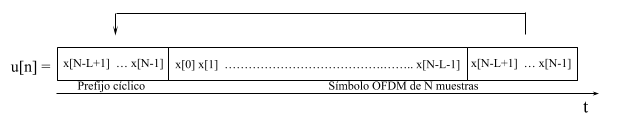
\includegraphics[scale=0.65]{figuras/cap03/prefijo_ciclico}
	\caption{\label{f:prefijo_ciclico} Inserción del prefijo cíclico.}
\end{figure}

Las últimas muestras del símbolo se copian al principio, de forma que al recibir, se calcula la autocorrelación del símbolo, que tendrá su pico en el comienzo de los datos válidos. Un ejemplo del prefijo cíclico se encuentra en la figura \ref{f:prefijo_ciclico}

La cantidad de muestras que se copian en el prefijo cíclico es un parámetro del sistema que los diseñadores pueden modificar según la aplicación. Generalmente se le denomina profundidad, y cuanto mayor sea la profundidad del prefijo, más robusto será el sistema frente a la \gls{ISI}, pero dejará disponible un menor ancho de banda.

La implementación de OFDM en los años 60 era prácticamente imposible, uno de los mayores problemas de los sistemas multiportadora, era la gran dificultad para escalar en cantidad de portadoras. La complejidad y el costo de construir los osciladores para la cantidad de canales necesarias, mantenían la brecha entre la teoría y la ejecución práctica. 

La solución a estos problemas, llegó cuando se logró programar computadoras capaces de procesar grandes cantidades de datos, mediante la implementación del algoritmo de “Fast Fourier Transform”. 

Weinstein y Ebert, resolvieron en  su publicación de 1971 \cite{discrete-ofdm} el mencionado problema de la escalabilidad, mediante la utilización de los avances tecnológicos de la época. Discretizando las señales a transmitir, y modulándolas por computadora, lograron formar sistemas multicanal para la transmisión en tiempo discreto en lugar de recurrir a los bancos de osciladores que se usaban hasta el momento. 

Su argumento provenía de la siguiente idea, una señal multitonal, puede ser vista como la transformada de Fourier de un tren de pulsos, y la demodulación coherente a su vez puede entenderse como la aplicación en tiempo continuo de una transformada inversa de Fourier. Entonces, probaron que muestreando la señal de origen, y mediante la implementación de un modem sobre una computadora que ejecute el algoritmo de la transofrmada rápida de Fourier, se pueden obtener aproximaciones suficientemente cercanas a los de la señal original. 

En síntesis, el esquema de un sistema transmisor OFDM tiene una forma similar a la presentada en la figura \ref{f:ofdm_system}. En la misma, el bloque \gls{CP} identifica la inserción del prefijo cíclico, y el bloque \xcancel{CP} identifica la remoción del mismo por parte del receptor.

\begin{figure}[h!]
	\centering
	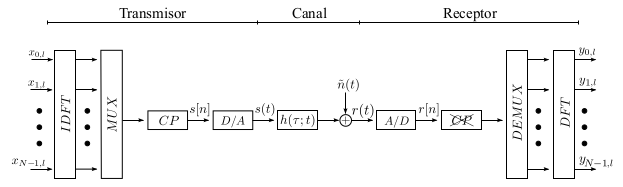
\includegraphics[scale=0.65]{figuras/cap02/ofdm_system}
	\caption{\label{f:ofdm_system} Esquema básico de un sistema OFDM.}
\end{figure}


\section{Codificación de canal}

	\subsection{C\'odigos de detecci\'on y correci\'on de errores}

La comunicación entre emisor y receptor puede modelarse mediante el proceso de la Figura \ref{diagrama_codificacion}. La situación es la siguiente, una fuente emisora envía mensajes $m$ (palabras fuente) al receptor a través de un canal de comunicación. El mensaje debe ser traducido a algún mensaje que el canal esté capacitado para enviar, estos mensajes se conocen como palabras código.

\begin{figure}[h!]
\centering
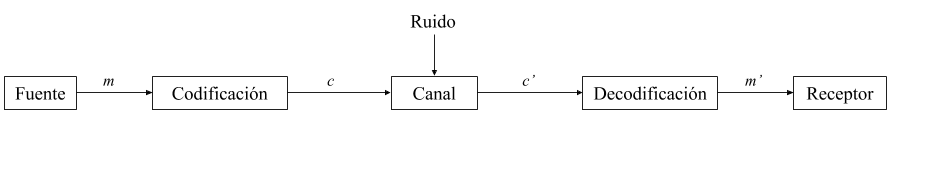
\includegraphics[scale=0.45]{figuras/cap02/diagrama_codificacion}
\caption{\label{diagrama_codificacion} Esquema básico de codificación de canal.}
\end{figure}

Al otro lado del canal llega un mensaje codificado $c'$, el cual seguramente sea erróneo, pues en todo proceso real de comunicación existe ruido e imperfecciones en los canales. El mensaje es decodificado en una palabra $m'$, y generalmente $m' \neq m$.

Se desea que el receptor sea capaz de darse cuenta si el mensaje $m'$ es realmente lo que se transmitió del otro lado, y más aún, poder corregirlo. 

La Teoría de Códigos es un campo de la matemática aplicada que busca resolver los problemas de las etapas de codificación-decodificación y corrección, y que presenta su propia complejidad.

La transmisión inalámbrica de una señal la expone a diversas fuentes de ruido, con lo cual los tipos de errores generados pueden ser muy variados. Por ejemplo los errores en ráfaga, en los que un conjunto de bits consecutivos se ven alterados, son muy comunes en las comunicaciones inalámbricas. También podría suceder que el canal radioeléctrico presente distorsión en algunas portadoras en particular.

El estándar ISDB-T hace uso de distintas técnicas para la protección de los datos en transmisión. De hecho para proteger los datos en los ejemplos mencionados el estándar utiliza las técnicas de \textit{entrelazamiento de bits y bytes} y la aplicación de códigos \textit{forward error correction} o FEC como es el caso de Reed Solomon. Para la comprensión del estándar y el desarrollo de \textit{gr-isdbt-tx} \cite{gr-isdbt-tx}, es importante conocer el funcionamiento de estas técnicas. Profundizar en estos temas escapa los objetivos de este trabajo, por lo cual los detalles técnicos se pueden encontrar en las bibliografías mencionadas.


\subsection{Códigos Cíclicos}
El conjunto $GF(2) \triangleq \{0,1\}$, con las operaciones de suma $" + "$ y producto $" \times "$ usuales módulo 2, cumple con la propiedad de que cualquier elemento de $GF(2)$ distinto de cero tiene inverso. Esta propiedad se cumple trivialmente en este conjunto y es la condición necesaria para que $GF(2)$ sea un \textit{Campo de Galois}. Es común encontrar que a este campo también se lo llame \textit{campo binario} y se lo denote como $\mathbb {F}_2$.
Las operaciones de suma y producto definidas en $GF(2)$ son asociativas, conmutativas y distributivas, y llevan elementos de $GF(2)$ en elementos de $GF(2)$. Por esto $GF(2)$ también es un \textit{anillo}. 
El conjunto de todos los polinomios con coeficientes en $GF(2)$ con las operaciones usuales de suma y producto forman un \textit{anillo de polinomios} en $GF(2)$ y se denota como $GF(2)[x]$. Por ejemplo $g(x) = x^3 + x + 1$ es un elemento de $GF(2)[x]$.

Sea $\textbf{c} = (c_0, c_1, ..., c_{n-1}) \in GF(2)$, con $GF(2)$ tal como se describió anteriormente. Un código $\mathcal{C}$ de bloque $(n, k)$ se dice que es un \textit{código cíclico} si para cada vector $\textbf{c} = (c_0, c_1, ..., c_{n-1}) \in \mathcal{C}$ cualquier rotación circular a la derecha de $C$ también pertenece a $\mathcal{C}$, es decir $(c_{n-1}, c_0, c_1, ..., c_{n-2}) \in \mathcal{C}$.
Los códigos de bloque se caracterizan por codificar mensajes de longitud fija $k$ en \textit{codewords} de longitud fija $n$, con lo cual el tamaño del mensaje original se incrementa en $n-k$.
Cada \textit{codeword} del código $\mathcal{C}$ puede ser representada en una forma polinomial de la siguiente manera:

\begin{equation}
c(x) = \sum_{i = 0}^{n-1}c_i x^i
\end{equation}

A continuación se enumera una serie de propiedades de los códigos cíclicos, en \cite{moon2005error} se puede encontrar una demostración detallada de cada una de ellas.

\begin{itemize}
\item{Un código cíclico es un código lineal de bloque}
\item{Cada \textit{codeword} se corresponde con un polinomio}
\item{Los polinomios del código forman un \textit{ideal} en $GF(2)[x]/(x^n-1)$}
\item{Para un código cíclico existe un generador $g(x)$ que es divisor de $x^n-1$ y que puede generar todos las \textit{codewords} $c(x)=m(x)g(x)$}
\end{itemize}

Se puede probar que esto implica la existencia de una \textit{matriz de chequeo de paridad} $\mathbb{H} \in \mathcal{M}_{(n-k)\times n}$ tal que para toda \textit{codeword} \textbf{c} de $\mathcal{C}$ se cumple $\textbf{c} \mathbb{H} ^T = \textbf{0}$.


El proceso de codificación se realiza de la siguiente manera. Primero se construye el polinomio $x^{n-k}m(x)$ de grado $n$. Luego se divide entre el polinomio generador $g(x)$ y el resto de esa división es el polinomio de paridad $d(x)$ que se le agregará al mensaje:

\begin{equation}
x^{n-k}m(x) - q(x)g(x) = d(x)
\end{equation}

La \textit{codeword} se forma de la siguiente manera:

\begin{equation}
c(x) = x^{n-k}m(x)-d(x) = q(x)g(x)
\end{equation}

Como se trata de un múltiplo de $g(x)$, entonces efectivamente es una \textit{codeword} válida. La representación vectorial de la \textit{codeword} queda de la siguiente manera:

\begin{equation}
\textbf{c} = (-d_0, -d_1, ..., -d_{n-k-1}, m_0, m_1, ..., m_{k-1})
\end{equation}

En una situación en la que se recibe una palabra $\textbf{r}$ cuyo mensaje es $\textbf{m}$  y sus bits de paridad son $\textbf{d}$, el procedimiento para detectar si hubo error es codificar el mensaje $\textbf{m}$ que se recibió con el mismo codificador utilizado por el transmisor (ambas partes deben conocer el polinomio generador), y luego comparar el $\textbf{d'}$ obtenido con el $\textbf{d}$ recibido. Si ambos difieren entonces hubo error. 
Por ejemplo, para un código cíclico (7, 4) con polinomio generador $g(x) = x^3 + x + 1$ se desea codificar el mensaje 1001. Los mensajes codificados tendran $n-k = 7 - 4 = 3$ bits de paridad. El mensaje en su forma polinomial queda $m(x) = 1 + x^3$.
Los bits de paridad se obtienen calculando el resto de la division $x^{(7-4)}m(x)/g(x)$, los coeficientes de ese resto seran los bits de la paridad buscada. Operando se llega a que la paridad es 011 y el mensaje codificado queda 0111001.

\subsection{Códigos Convolucionales}

Los \textit{códigos convolucionales} son un tipo de códigos lineales que debido a su estructura, la codificación mediante estos códigos puede ser vista como un proceso de filtrado o convolución, de ahí su nombre. 

A diferencia de los códigos de bloque que toman bloques de k-símbolos y devuelven bloques de n-símbolos, los códigos convoulcionales funcionan como códigos de flujos. Esto significa que operan en flujos continuos de símbolos y no en paquetes discretizados. De hecho se define la tasa del código como el cociente $k/n$.

El funcionamiento del codificador convolucional consiste en una serie de $k$ registros inicializados en algún valor. La salida de cada uno de estos registros ingresa a $n$ sumadores binarios (\textit{xor}). Los registros que intervienen en cada operación de suma están determinados por los polinomios generadores. Cada rama tiene asociada un polinomio generador y es común encontrar que se refiere a ellos en notación octal. Por ejemplo ISDB-T utiliza $G_1 = 171_{OCT} (1111001_b)$ y $G_2 = 133_{OCT} (1011011_b)$, significa que $G_1$ utiliza el bit de entrada, los primeros tres registros y el último registro. 

\subsection{Códigos de Reed-Solomon}

Los códigos de Reed-Solomon son un tipo de códigos FEC no binario que corrigen los datos erróneos recibidos durante una transmisión. Se caracterizan por utilizar símbolos en lugar de bits, es decir que un conjunto de $m$ bits consecutivos forman un símbolo. Se dice que el símbolo es erróneo si al menos un bit del símbolo es incorrecto. Las palabras del código estan formadas por $n = k +r $ símbolos, donde $r$ son de paridad. La longitud del bloque de información es $r$ y el código es capaz de corregir hasta $r/2$ símbolos erróneos. 
Debido a su capacidad de corrección de errores son especialmente indicados para tratar los errores en ráfagas.



\section{La entrada de datos a ISDB-T}

\subsection{MPEG}

El Moving Picture Experts Group (MPEG)\cite{MPEG} es un grupo de trabajo conformado por expertos internacionales, formado por la Organización Internacional de Normalización (ISO) en conjunto con la Comisión Electrotécnica Internacional (IEC), con el objetivo de desarrollar estándares para la codificación, compresión y transmisión de audio y video.

Uno de los estándares publicados por el MPEG, es MPEG-2. Consta de métodos para la compresión digital de contenidos audiovisuales,  y abarca la difusión de los mismos a través de una amplia gama de tecnologías, desde el streaming de datos a través de la web, codificación de voz y video para telefonía y videoconferencias, comercialización de discos compactos (\gls{CD}) y hasta formatos para la transmisión de televisión. 

Es en este último punto donde se vincula con ISDB-T Internacional, puesto que para la codificación de fuente en la norma, fue seleccionado el Estándar MPEG-4 Parte 10 “Advanced Video Coding”, también denominado H.264 \cite{mpeg4_10}.

Para garantizar que los receptores de televisión digital ISDB-T también sean compatibles con los transmisores tanto de ISDB-T como de ISDB-T International, se encapsulan los videos codificados en H.264 dentro de un formato denominado “Transport Stream” que se define en la norma MPEG-2 Parte 1 – Sistemas \cite{mpeg2_1}.

En el transmisor gr-isdbt-tx, tomamos como fuente de datos un archivo codificado como Transport Stream, para garantizar esta compatibilidad.

	\subsection{MPEG 2 Transport Stream}
	
	A la hora de transmitir televisión, los datos a transmitir son un conjunto de lo que se denomina \textit{programas}, que son datos de video, audio, ocasionalmente subtítulos y otros datos de interés del broadcaster.  
	
	Cada programa es comprimido de forma independiente, formando lo que se denomina \textit{Elementary Stream (\gls{ES})} o flujo elemental. Para poder ser multiplexados y transmitidos, los ES se paquetizan para formar estructuras denominadas \textit{Packetized Elementary Stream (PES)}. Dependiendo del tipo de transmisión a realizar, los PES pueden sufrir dos tipos de modificaciones. En caso de orientarse a un entorno poco ruidoso, los \gls{PES} se codifican en los llamados Program Streams, que en general son contenedores donde los paquetes de datos pueden ser de tamaño y bitrate variable. En caso de que la transmisión sea a través de un medio muy ruidoso, como es el caso de la televisión digital terrestre, los PES deben ser codificados en los llamados \textit{Transport Streams}. Básicamente, para convertir un PES a un \gls{TS} se reduce el tamaño de los paquetes a un contenedor fijo de 188 bytes, sobre los cuales se ejecutaran posteriormente códigos correctores de errores de tipo \gls{FEC}, como los vistos en la sección anterior.
	
	Al comienzo de la cadena de transmisión, en ISDB-T, se multiplexan varios TS, junto con tablas de información que contienen la información y posición de los programas en el flujo. Se crea entonces un único TS de transmisión sobre el cual se van a realizar las tareas de codificación, robustecimiento ante pérdidas y posteriormente la modulación y otras técnicas que se verán mas adelante.
	
	Cuando un receptor obtenga el TS en cuestión, no tendrá en principio información alguna sobre el contenido del flujo. Dicha información existe en las tablas, pero en un momento inicial de la recepción, tampoco están disponibles puesto que están multiplexadas con todos los demás paquetes del TS. Cada paquete contiene un identificador único denominado Packet Identifier (\gls{PID}). Como las tablas contienen información vital para la decodificación, sus números PID son bien conocidos por el receptor, de forma que puede buscar entre todos los paquetes aquellos que le darán la información para comenzar la decodificación. La primera tabla que el receptor busca en el TS, es la tabla \gls{PAT}, que tiene asignado el PID 0x0000. 
	
	\subsection{Tabla PAT}
	La Program Association Table (PAT), es una tabla que contiene una lista de todos los programas disponibles en el TS. Está formada por valores de 16 bits denominados Program Number, asociados cada uno de ellos con el PID correspondiente a la tabla PMT de cada uno de los programas dentro del stream. 
	
	De este modo, el receptor que se conecta al stream en cualquier momento de la transmisión, lee la tabla PAT y obtiene un listado de los programas existentes en el TS y los PIDs de sus correspondientes PMTs. 

	\subsection{Tablas PMT}

	Cada programa del TS tiene su tabla PMT (Program Map Table), identificada tambien por su PID único. En la tabla PMT, esta la información correspondiente a los PIDs de los paquetes que pertenecen al programa en cuestión.
	
	Una vez obtenida la tabla \gls{PMT} del programa que se desea decodificar, el receptor debe almacenar los PIDs que estan contenidos en ella. Luego, basta con filtrar los paquetes del TS para obtener solo los datos del programa a decodificar. 
		
	Además de la tabla PAT y las PMT, existen otros tipos de tablas en MPEG-2. Para el alcance de este documento, con la descripción de estas dos es suficiente, pero si nos interesa destacar otro tipo de paquete del TS con un PID bien conocido.
	
	\subsection{Paquetes Nulos}
	
	Resulta vital para un esquema de transmisión de televisión mantener el bitrate constante, puesto que esto mantiene el ancho de banda de tamaño constante. En una transmisión de datos multimedia, hay variabilidad en la tasa de bits todo el tiempo, por lo que puede ocurrir que en algún momento falten datos para contemplar esa tasa. Es por eso que se definen los paquetes nulos. Un multiplexor completa con paquetes ``dummy`` cuando ocurre esta deficiencia, y así logra para mantener la tasa constante. El PID de los paquetes nulos es el 0x1FFF.
	
\subsection{Broadcast Transport Streams}

El estándar MPEG no está pensado para la transmisión en capas jerárquicas. Para lograr la característica de la transmisión jerárquica y la recepción parcial, ISDB-T cuenta con una solución propia denominada Broadcast Transport Stream. Esta solución consiste en el uso
de un flujo de transporte propio, formado a partir de tres flujos MPEG multiplexados, lo que supone un procesamiento no tan sencillo. El nuevo flujo deberá incluir cierta información jerárquica, que no provee MPEG, que permita identificar los flujos con sus correspondientes capas jerárquicas. Es importante que el sistema funcione a una velocidad de reloj constante y determinada, por este motivo el flujo BTS deberá tener una tasa perfectamente definida y constante independientemente de los parámetros de cada capa.

La conformación del \gls{BTS} se lleva a cabo en el bloque TS Remux. Es el encargado de agregar 16 bytes al final de cada paquete TS con la ISDB-T information y la paridad; posicionar los TSP dentro del BTS de acuerdo a cierto patrón de ordenamiento que se detallará, para posibilitar la transmisión jerárquica; insertar la cantidad necesaria de paquetes nulos para asegurar una tasa constante $r_{BTS}$. 

\begin{equation*}
	r_{BTS} = 4 \times f_{IFFT} = \frac{2048}{63} \approx 32.508 \quad Mbps
\end{equation*}

La obtención de la fórmula anterior, en conjunto con una descripción mas detallada del Multiplex Frame para ISBD-T puede encontrarse en el análisis realizado por Pablo Flores y Federico La Rocca en \cite{gr-isdbt}.

Durante la división jerárquica la ISDB-T information de los TSP es removida por lo cual en las siguentes fases de procesamiento ya no se cuenta con la información jerárquica en los flujos de transporte. Es por eso, que resulta necesario definir un orden predefinido dentro del BTS de manera que el receptor pueda reconstruirlo perfectamente sin necesidad de la ISDB-T information. 

Supongamos que tenemos un BTS como el de la figura \ref{f:bts1} en el cual hay dos capas jerárquicas A y B, cada una con su respectiva tasa tal que $r_{BTS}> r_B > r_A$. Las capas con tasas altas implican un tiempo de transmisión de paquetes mucho más corto que las capas con tasas bajas, y viceversa.

\begin{figure}[h!]
	\centering
	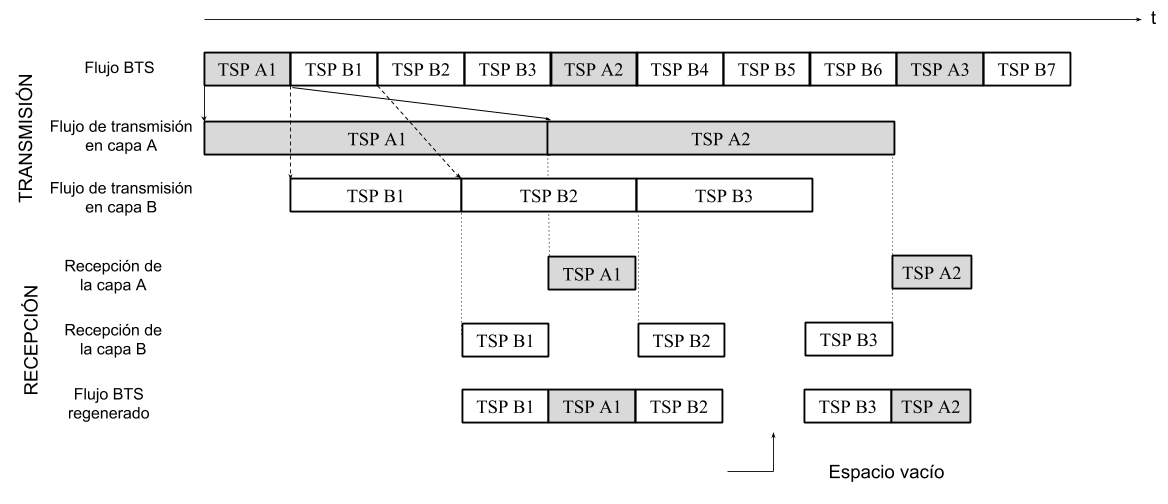
\includegraphics[scale=0.35]{figuras/cap02/bts1}
	\caption{\label{f:bts1} Patrón de ordenamiento incorrecto del BTS.}
\end{figure} 

Observando el diagrama de la figura \ref{f:bts1} puede verse que en recepción el paquete $B_1$ es procesado antes de que termine de ser transmitido el paquete $A_1$, cuando en realidad el orden original era $A_1$ y luego $B_1$. Además se generan espacios de tiempo en los cuales no se entregan paquetes al sistema porque aún se están procesando paquetes que van arribando. Esos intervalos de tiempo deben ser rellenados con paquetes nulos a fin de mantener la tasa constante. Esto resulta en un desordenamiento del patrón original del BTS y de la pérdida total de la capacidad de reordenar los datos en recepción.

Para formar los patrones de ordenamiento en transmisión de manera tal que el receptor sea capaz de recuperarlos perfectamente, se agregan los denominados ajustes de atraso. En el ejemplo de la figura \ref{f:bts2} se agrega un ajuste de atraso de 2 TSP y se introduce un paquete nulo en el BTS original. Como resultado, el flujo BTS reconstruído por el receptor resulta ser exactamente igual al BTS original. Dada una configuración jerárquica del sistema, existe un único patrón de ordenamiento del BTS.

El transmisor implementado en este trabajo toma como flujo de entrada un BTS ya conformado, y con la información jerárquica de los TSP es que logra procesar cada capa por separado. De ahí en adelante las capas son entrelazadas y moduladas cada una de acuerdo a su propia configuración.

\begin{figure}[h!]
	\centering
	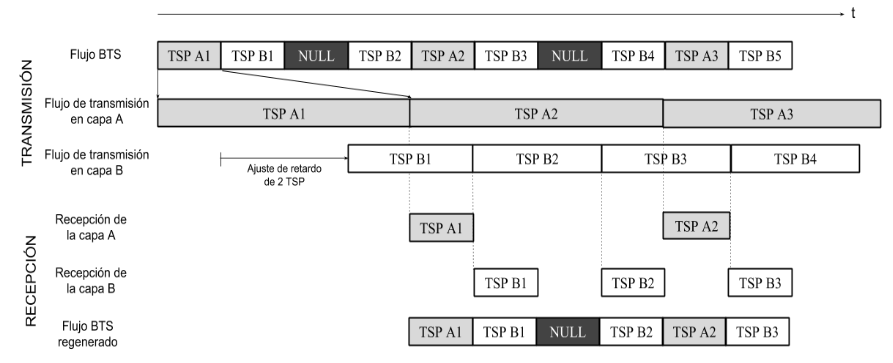
\includegraphics[scale=0.45]{figuras/cap02/bts2}
	\caption{\label{f:bts2} Patrón de ordenamiento correcto del BTS.}
\end{figure}